\begin{figure}[H]
  \centering

  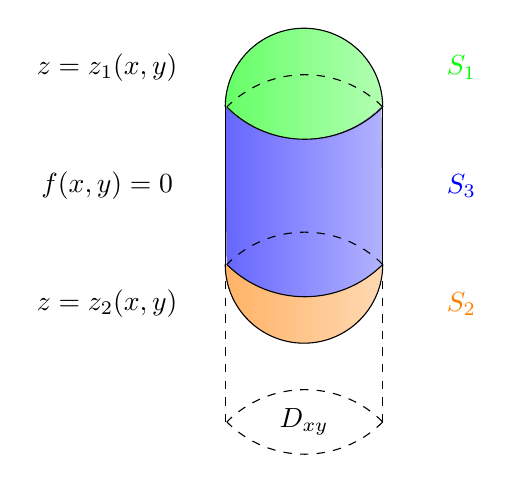
\begin{tikzpicture}
    \fill[left color = green!60, right color = green!30]
      (-1, 2) arc (225 : 315 : 1.4)
      -- (1, 2) arc (0 : 180 : 1)
      -- cycle;

    \fill[left color = blue!60, right color = blue!30]
      (-1, 2) arc (225 : 315 : 1.4)
      -- (1, 0) arc (-45 : -135 : 1.4)
      -- cycle;
  
    \fill[left color = orange!60, right color = orange!30]
      (1, 0) arc (-45 : -135 : 1.4)
      -- (-1, 0) arc (180 : 360 : 1)
      -- cycle;

    \draw (-1, 0) -- (-1, 2);
    \draw (1, 0) -- (1, 2);

    \draw[dashed] (1, 2) arc (45 : 135 : 1.4);
    \draw (1, 2) arc (-45 : -135 : 1.4);
    \draw[dashed] (1, 0) arc (45 : 135 : 1.4);
    \draw (1, 0) arc (-45 : -135 : 1.4);

    \draw (1, 2) arc (0 : 180 : 1);
    \draw (1, 0) arc (0 : -180 : 1);

    \draw[dashed] (1, 0) -- (1, -2);
    \draw[dashed] (-1, 0) -- (-1, -2);

    \draw[dashed] (1, -2) arc (45 : 135 : 1.4);
    \draw[dashed] (1, -2) arc (-45 : -135 : 1.4);
    \draw node at (0, -2) {\(D_{xy}\)};

    \draw node at (2, 2.5) {\textcolor{green}{\(S_{1}\)}};
    \draw node at (2, 1) {\textcolor{blue}{\(S_{3}\)}};
    \draw node at (2, -0.5) {\textcolor{orange}{\(S_{2}\)}};

    \draw node at (-2.5, 2.5) {\(z = z_{1}(x, y)\)};
    \draw node at (-2.5, 1) {\(f(x, y) = 0\)};
    \draw node at (-2.5, -0.5) {\(z = z_{2}(x, y)\)};

  \end{tikzpicture}
\end{figure}
